It is essential for all modern collider experiments to have an online monitoring of the beam conditions. Since it is important to have these detectors as close as possible to the beam all of the four main experiments at the \ac{LHC} are using detectors with diamond sensors. ATLAS \cite{gorisek}, ALICE, CMS \cite{bartz} and LHCb \cite{domke} all make use of various \acp{BCM} and/or \acp{BLM} based on both \ac{CVD} type diamonds for live background estimations and luminosity measurements.\\
As an upgrade of the \ac{BCM} during the long shutdown in 2014 ATLAS installed the \ac{DBM}. Its purpose is to measure an instantaneous (bunch-by-bunch) luminosity and the bunch-by-bunch position of the beam spot. With its eight telescopes à three detector planes it adds tracking capability to the existing precise \ac{ToF} measurements of the eight pad detectors of the \ac{BCM}. The usage of state of the art pixel detectors based on the FE-I4b readout chip strongly increases the spatial resolution of the monitor and due to its projective geometry pointing towards the interaction region it also can distinguish particles coming from collisions and background \cite{dbm}. The telescopes whereof the sensors of two are made out silicon and the other six out of \ac{p}\ac{CVD} diamond are positioned symmetrically around the beam pipe on both sides of the interaction point and are shown in \vref{dbm}.
\begin{figure}
	\centering
	\begin{subfigure}{.66\textwidth}
		\centering
		\vspace*{.05\textheight}
		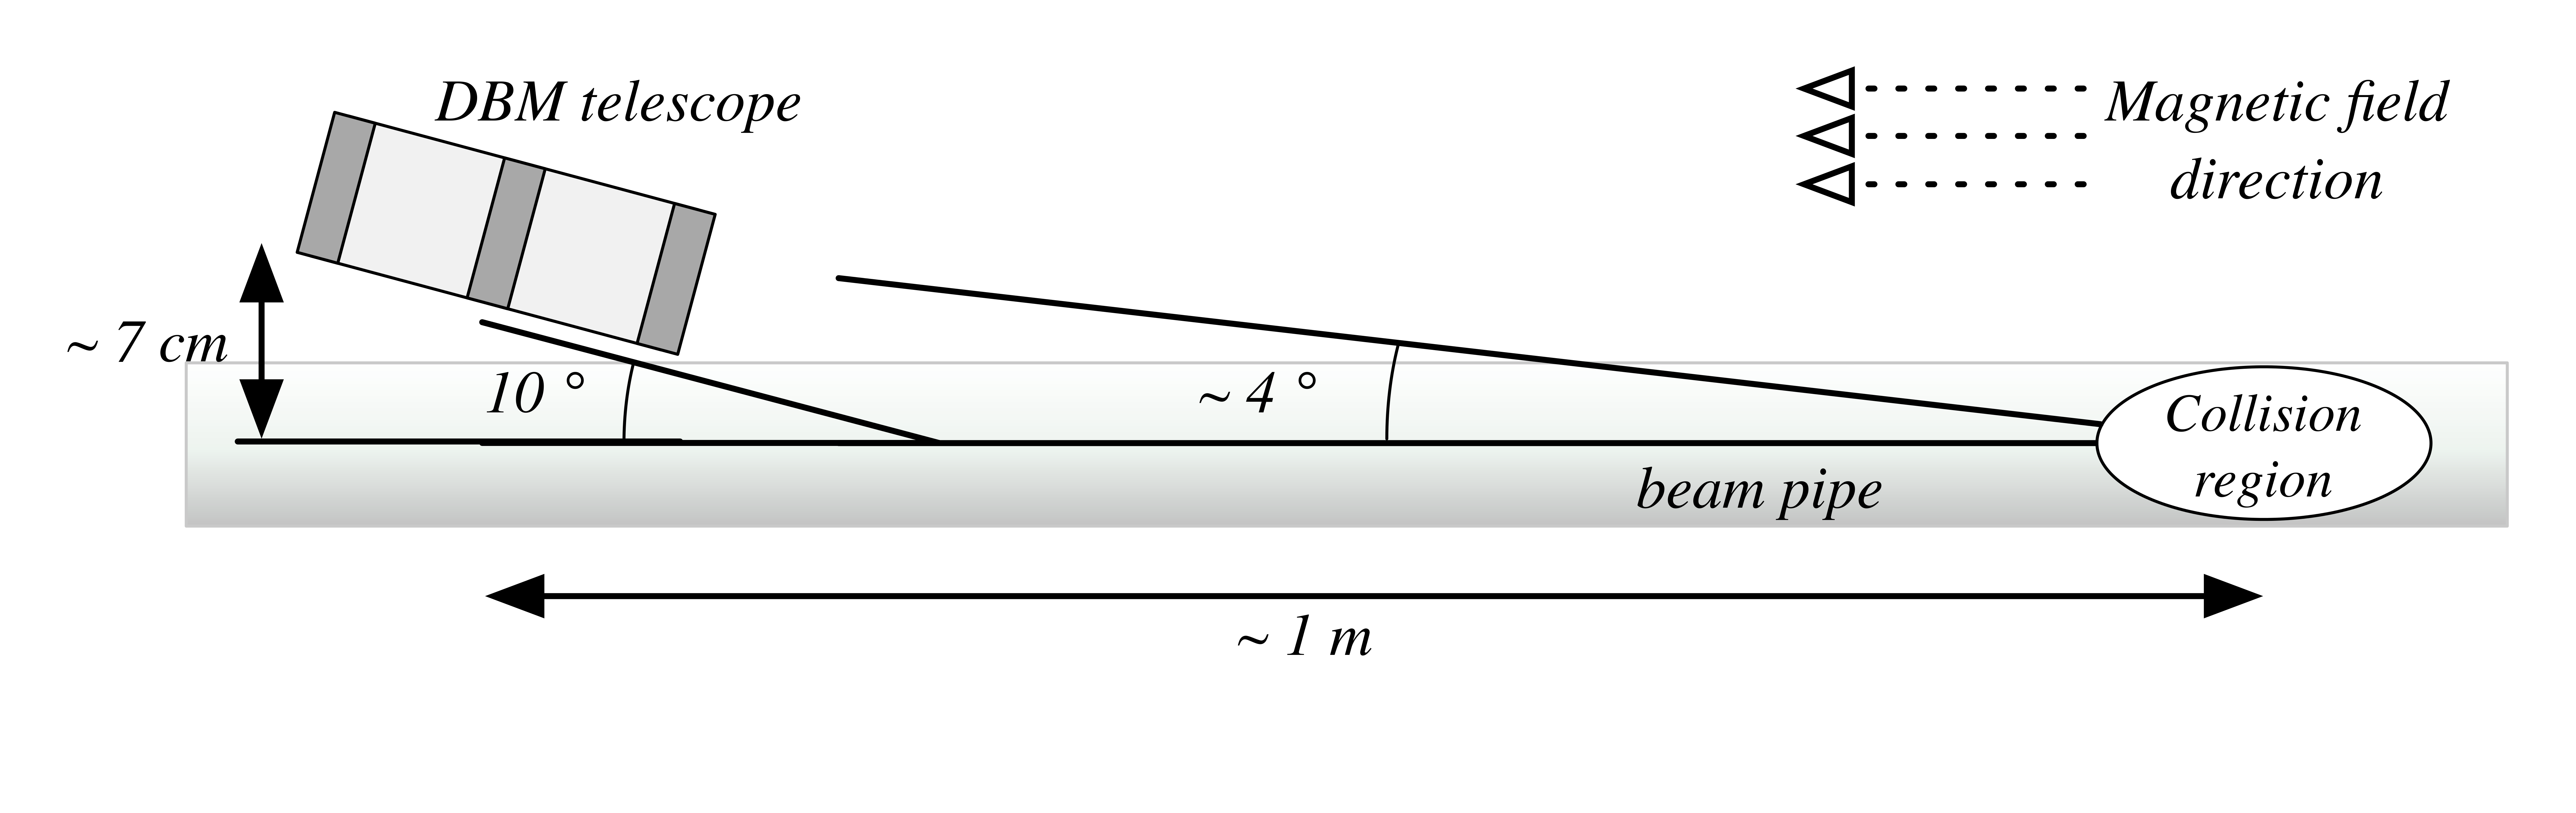
\includegraphics[height=.14\textheight]{dbm1.png}
		\vspace*{.02\textheight}
		\caption{positioning and alignment}
	\end{subfigure}
	\subfig[.33]{DBM2.png}{.23}{four mounted telescopes}
	\caption{\ac{DBM} telescope}
	\label{dbm}
\end{figure}
